\chapter{Empirical Evaluation and Results}
\label{chap:experiments}

\section{Experimental Setup}
To assert the superiority of the Green AI paradigm, we submitted both the conventional delay-centric D3QN agent and the emission-aware Green D3QN agent to a battery of deterministic simulation episodes. Employing synchronized randomized seeding ensured that both agents faced perfectly identical vehicle spawn patterns, exact routing demands, and matching traffic surge intensities.

\section{Quantitative Performance Comparison}
The resulting analytical metrics demonstrate that inserting a carbon penalty forces the neural network to uncover a strictly superior global handling strategy that evades cascading failures. Table~\ref{tab:traffic_metrics} illustrates the traffic-flow outcomes.

\begin{table}[h]
\centering
\caption{Traffic Performance Metrics}
\label{tab:traffic_metrics}
\renewcommand{\arraystretch}{1.2}
\begin{tabular}{|l|c|c|c|}
\hline
\textbf{Traffic Metric} & \textbf{Standard DRL Agent} & \textbf{Green AI DRL Agent} & \textbf{Improvement} \\
\hline
Mean Waiting Time & $125.54 \pm 223.94$ s & $17.53 \pm 4.59$ s & -86.0\% \\
Mean Time Loss & $151.18 \pm 257.22$ s & $25.50 \pm 4.68$ s & -83.1\% \\
Mean EMV Delay & $292.66 \pm 585.33$ s & $0.00 \pm 0.00$ s & -100.0\% \\
\hline
\end{tabular}
\end{table}

\section{Environmental and Chemical Reductions}
As demonstrated in Table~\ref{tab:emissions}, the Green AI agent successfully curtails total vehicle emission footprints.

\begin{table}[h]
\centering
\caption{Environmental and Chemical Reductions}
\label{tab:emissions}
\renewcommand{\arraystretch}{1.2}
\begin{tabular}{|l|c|c|c|}
\hline
\textbf{Emission Metric} & \textbf{Standard DRL Agent} & \textbf{Green AI DRL Agent} & \textbf{Improvement} \\
\hline
CO\textsubscript{2} Mass (kg) & $18.92 \pm 9.08$ & $14.68 \pm 0.60$ & -22.4\% \\
NOx Mass (g) & $8.07 \pm 4.19$ & $6.11 \pm 0.28$ & -24.3\% \\
PMx Mass (g) & $0.39 \pm 0.23$ & $0.29 \pm 0.02$ & -27.5\% \\
Fuel Burn (Liters) & $6034.69 \pm 2894.78$ & $4681.38 \pm 192.51$ & -22.4\% \\
\hline
\end{tabular}
\end{table}

\section{Evaluation of Systemic Stability and Gridlock}
The massive standard deviation ($\pm 223.9$ s) attached to the Standard agent's wait time highlights a critical vulnerability in traditional formulations: in demanding traffic scenarios (such as localized traffic spikes seen during evaluation), the wait-optimized agent induced catastrophic system failure, commonly classified as gridlock, inflating average episode wait times up to nearly 600 seconds. 

By contrast, the Green AI agent exhibited virtually zero variance ($\pm 4.5$ s) across the identical challenges. Because a stagnant intersection produces astronomical cumulative exhaust readouts, the agent discovered that anticipating flow and avoiding stop-and-go blockage was biologically imperative for minimizing its loss function. In effect, penalizing CO\textsubscript{2} yielded a secondary mechanism for unshakeable traffic fluidity.

\section{Visual Performance Verification}
Figure~\ref{fig:charts} provides a visual comparison of the evaluation metrics between the two policies.

\begin{figure}[h]
\centering
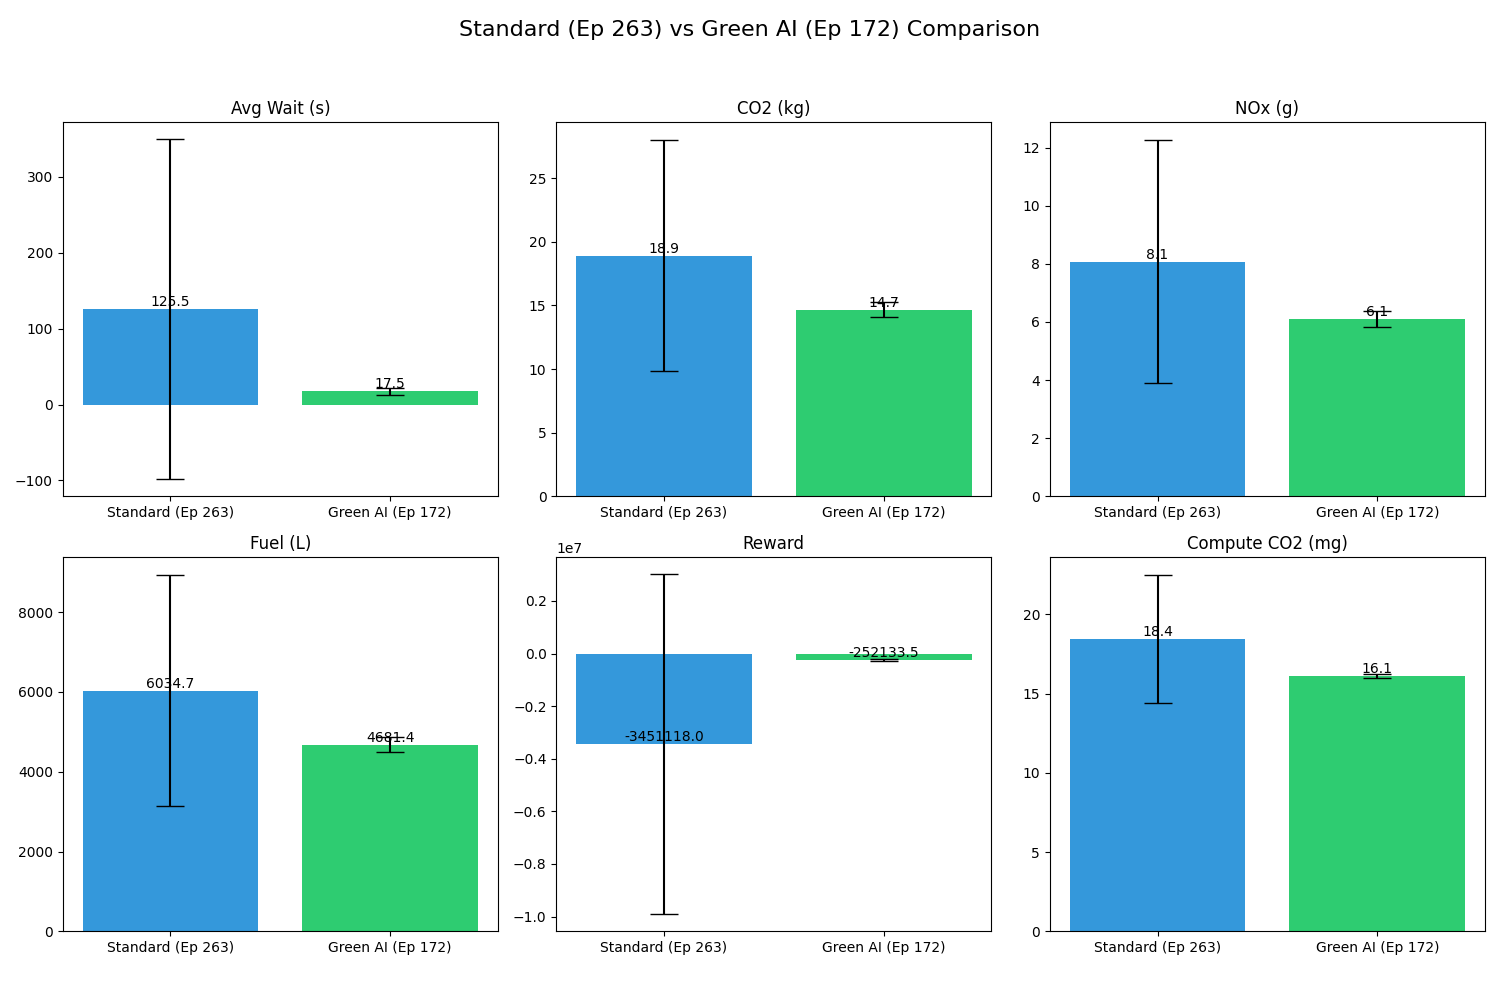
\includegraphics[width=0.8\textwidth]{comparison_charts.png}
\caption{Benchmark Comparison Charts evaluating the Standard and Green AI configurations across identical traffic scenarios.}
\label{fig:charts}
\end{figure}

\section{AI Hardware Footprint vs. Saved Exhaust}
The mean computational carbon expenditure produced by running inference for the Green AI algorithm across the 2x2 grid averaged to merely $16.10$ mg CO\textsubscript{2} per episode. When contrasted with the macroscopic savings of over $4.24$ kilograms of tailpipe CO\textsubscript{2} avoided per equivalent timeframe, the carbon-cost of executing the AI yields an overarching return on investment surpassing a ratio of 1:260,000, wholly validating the Green AI proposition.